\section{Experimental analysis}
  
\subsection{Event reconstruction}

For this analysis a simplified simulation of detector response and  object reconstruction is used. Objects are required not to overlap with each other.
Leptons (electron and muons) are required to originate from a $W$-boson or $\tau$-lepton decay and to have $\pt >25$ \gev and $|\eta|<2.5$. To mimic the typical performance of an LHC detector, a reconstruction efficiency of $80\%$ is assumed. A simplified simulation of a calorimeter is used to build jets.  The four momenta of stable particles, except muons and neutrinos, falling within the same window in $\eta-\phi$ space of size $\Delta \eta \times \Delta \phi = 0.1 \times 0.1$ are added together to simulate the granularity of calorimeter cells.  For each cell, the total three momentum is rescaled such as to make the cell massless.  Cells with energy larger than 0.1 $\gev$ and $|\eta|<5.0$ become the inputs to the jet algorithm. Four jets collections are considered in this analysis. All jets contained in the four collections are required to satisfy $|\eta|<2.5$. For those collections a semi-muonic energy correction is applied to recover the significant fraction of energy carried away by muons in $b$-hadron decays. This correction adds to to the calorimeter jet four momentum the four momenta of all reconstructed muons with $\pt>4$ $\gev$ that are ghost-associated to a jet. \par Two jet collections are built using the anti-$k_{\rm T}$ algorithm with two different radius paramenter, $R$=0.2 and $R$=0.4, referred to as AKT2 and AKT4 jets respectively.
A minimum \pt requirement of 15 and 25 $\gev$ is made for AKT2 and AKT4 respectively. AKT4 jets are used to define the jet multiplicity of the event, while AKT2 are chosen to define the $b$-tag multiplicity of the event since at low $m_{A}$ values the $b$-quarks from the $A\to b \bar{b}$ decay emerge with small angular separation (see figure \ref{sec:ttA:fig:drbb}).
\begin{figure}[htbp!]
\centering
\begin{subfigure}{0.45\textwidth}
  \centering
  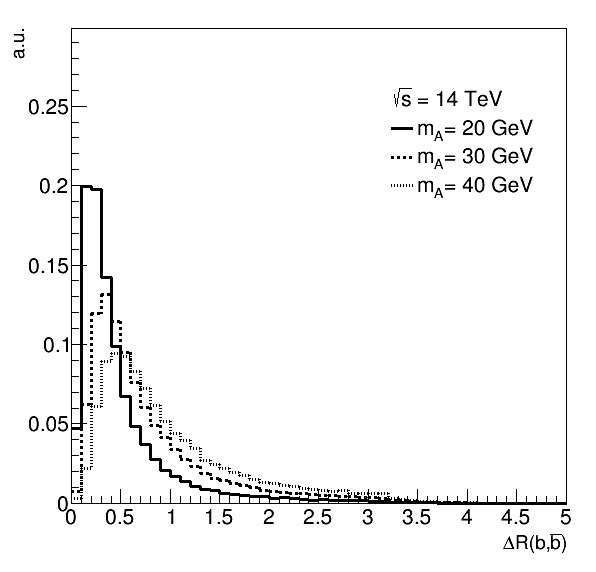
\includegraphics[width=0.9\textwidth]{figures/ttA/DRbb.png}
  \caption{}
  \label{}
\end{subfigure}
\begin{subfigure}{0.45\textwidth}
  \centering
  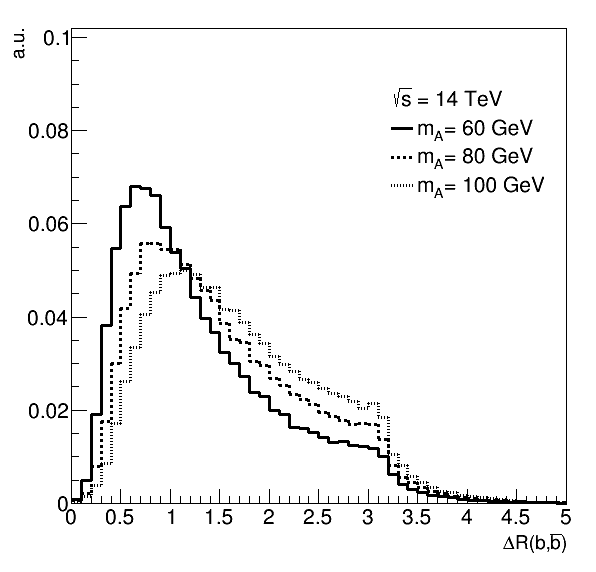
\includegraphics[width=0.9\textwidth]{figures/ttA/DRbb2.png}
  \caption{}
  \label{}
\end{subfigure}
\captionsetup{width=0.85\textwidth} \caption{\small Distribution of $\Delta R$ between the two $b$-quarks from the $A\to b \bar{b}$ decay prior to any selection requirements, for different
values of $m_{A}$: (a) $m_{A}$= 20, 30 and 40 \gev, and (b) $m_{A}$= 60, 80 and 100 \gev.}
\label{sec:ttA:fig:drbb}
\end{figure}
Heavy-flavour tagging is modelled in a probabilistic fashion by assigning a per-jet efficiency of $70\%$ to $b$-jets, $20\%$ to $c$-jets, and $0.7\%$ to light jets.  AKT2 jets are labelled as $b$-jet or $c$-jet if they are matched respectively to a $b$-hadron or a $c$-hadron (not originating from a $b$-hadron decay) within $\Delta R= 0.15$. The rest of the jets are taken to originate from the fragmentation of a light quark or gluon and are labelled as ``light  jets''.  \par The other two jet collections are reconstructed with the Cambridge-Aachen (C/A) algorithm, which corresponds to the choice of $p=0$ in the equations \ref{eq:obj:jets:d1} and \ref{eq:obj:jets:d2}. This algorithm clusters particles based exclusively on the spatial separation. The C/A algorithm is capable of discerning the components closest to the hard jet; it is
therefore well-suited to discriminating softer subjets within harder jets. Thus, C/A jets are used  to reconstruct the $A\to b \bar{b}$ decay, taking advantage of the boost with which $A$ bosons are produced in the $t\bar{t}A$ process.  Two radius parameters, $R$=0.6 and $R$=0.8 (referred to as CA6 and CA8 respectively), are chosen in order to optimise the reconstruction of the $A$ boson depending on the value of the mass $m_A$.
In order to minimise the impact of soft radiation and pileup (not modelled in this analysis), the mass-drop (a.k.a. BDRS) filtering algorithm \cite{Butterworth:2008iy} with the following parameters, $\mu_{\rm frac}=0.67$ and $y_{\rm cut}=0.09$ is applied to the reconstructed C/A jets. 


\subsection{Analysis strategy}

The final-state signature is characterised by one electron or muon and high jet and $b$-tag multiplicities. Therefore, events are required to satisfy the following requirements, referred to as ``preselection'': one electron or muon, $\ge5$ AKT4 jets and $\ge3$ AKT2 $b$-tagged jets (referred to as $\ge$5j, $\ge$3b). After the preselection $t\bar{t}+$jets is the dominant background. Following a similar strategy to those described in chapters \ref{chp:VLQ} and \ref{chp:ttH}, the events are categorised in two exclusive regions based on the number of $b$-tagged jets (3 and $\ge$4) in order to take advantage of the higher $b$-jet multiplicity of the signal process. \par The $\ge$ 5j, $\ge$4b region is dominated by $t\bar{t}+$HF-jets events but it  has the largest signal-to-background ratio and thus drives the sensitivity of the search.
The $\ge5$j, $3$b region instead has significantly lower signal-to-background ratio and the background is enriched in $t\bar{t}+$light-jets.
The simultaneous analysis of both channels gives the possibility to measure in-situ the $t\bar{t}$+jets background (including its heavy-flavour content) and constrain the related systematic uncertainties.\par
After event categorisation this analysis, compared to the $t\bar{t}H$ search described in chapter \ref{chp:ttH}, can make use of the boost of the $A$ boson to further suppress the background. The two $b$-jets from the $A$-boson decay are collimated, particularly at low $m_{A}$ mass, and can be reconstructed into a single fat jet, whose mass distribution would show a resonant structure peaked at the correct $m_{A}$ value. Therefore, events are required to have at least one C/A BDRS-filtered jet with radius parameter $R^{CA}$ and minimum $\pt$ depending on the $m_{A}$ hypothesis being tested. CA6 jets are used for $m_{A}<$ 40 \gev, while CA8 jets are used for higher $m_{A}$ values (up to 100 \gev). The minimum $\pt$ requirements on the C/A jets are 60, 100, 120, 150, 200, and 250 $\gev$ for $m_{A}$ = 20, 30, 40, 60, 80, and 100 $\gev$, respectively. The number of $b$-tags inside the C/A jet is determined by matching the $b$-tagged AKT2 jets within a cone of radius $R$= 0.75$R^{CA}$. Finally, it is required that the C/A jets have $\ge2$ $b$-tags inside. In case of more than one selected C/A jet, the leading-$\pt$ one is chosen. The final discriminating variable is the invariant mass of the selected C/A jet, referred to as ``leading BDRS jet mass'', shown in figure \ref{sec:ttA:fig:bdrsmass} for signal and background in each of the analysis channels, for two different values of $m_{A}$.


\begin{figure}[p!]
\begin{subfigure}{0.5\textwidth}
  \centering
  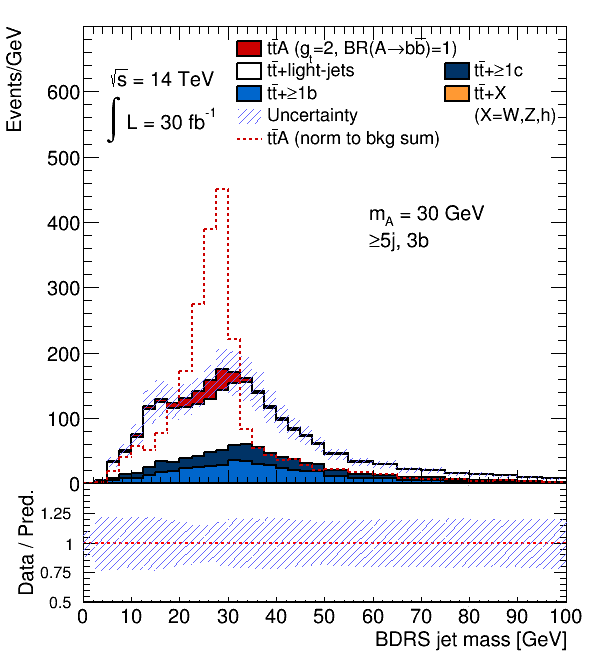
\includegraphics[width=0.9\textwidth]{figures/ttA/VD_1_30.png}
  \caption{}
  \label{}
\end{subfigure}
\begin{subfigure}{0.5\textwidth}
  \centering
  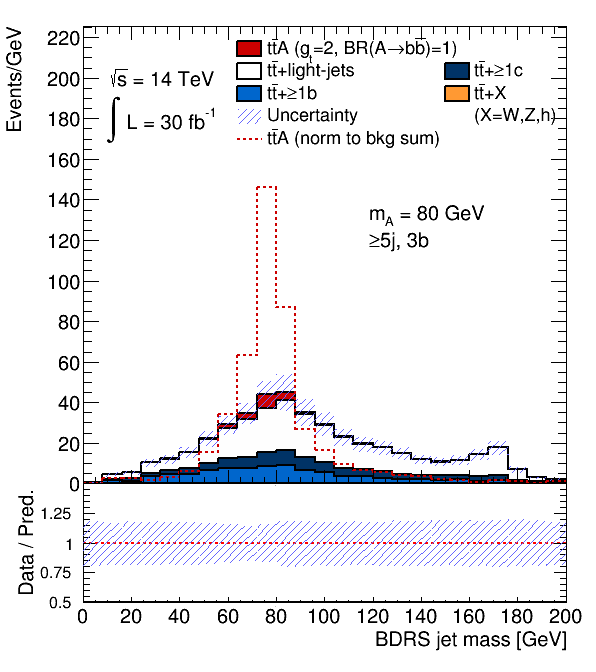
\includegraphics[width=0.9\textwidth]{figures/ttA/VD_1.png}
  \caption{}
  \label{}
\end{subfigure}
\begin{subfigure}{0.5\textwidth}
  \centering
  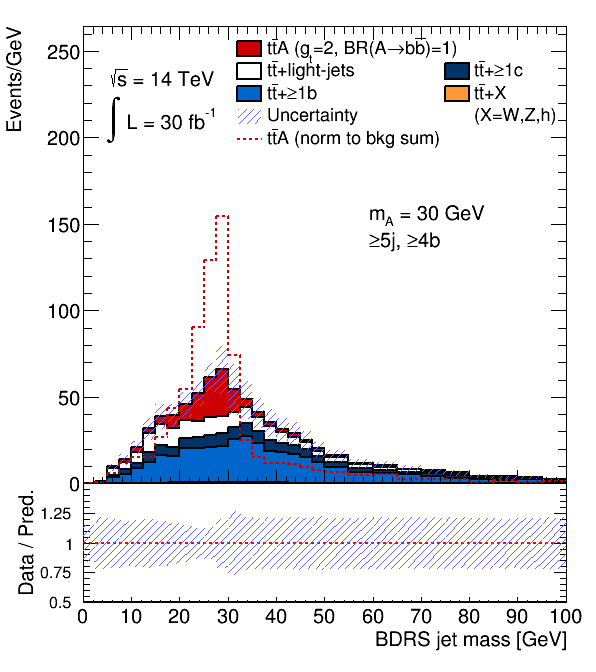
\includegraphics[width=0.9\textwidth]{figures/ttA/VD_2_30.png}
  \caption{}
  \label{}
\end{subfigure}
\begin{subfigure}{0.5\textwidth}
  \centering
  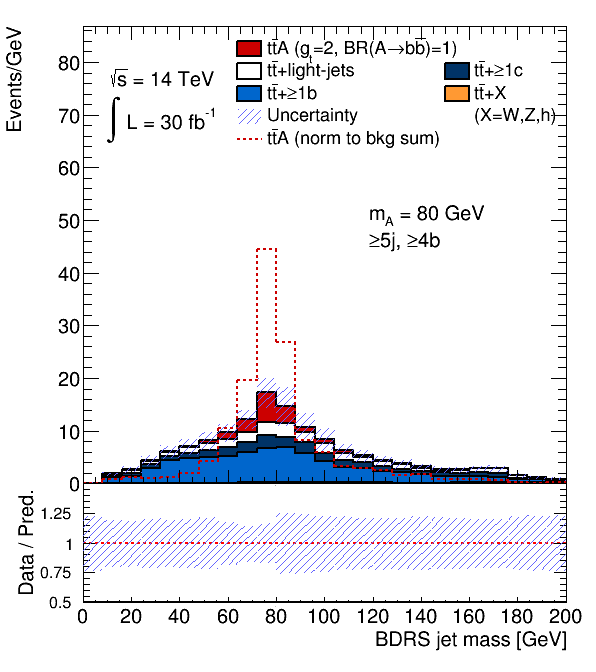
\includegraphics[width=0.9\textwidth]{figures/ttA/VD_2.png}
  \caption{}
  \label{}
\end{subfigure}
\captionsetup{width=0.85\textwidth} \caption{\small Distribution of the leading BDRS jet mass in the two analysis channels considered after final selection:  (a, b) ($\ge5$j, $3$b) and (c, d) ($\ge5$j, $\ge4$b), for different values of $m_{A}$ (30 and 80 \gev). The prediction corresponds to $\sqrt{s}=14$ $\tev$ and an integrated luminosity of 30 fb$^{-1}$.   Contributions from $t\bar{t}W$, $t\bar{t}Z$ and $t\bar{t}H$ have been merged for visibility. The expected contribution from the $t\bar{t}A$ signal under the assumptions of $g_{t}= 2$ and ${\rm BR}(A\to b\bar{b})=1$ is also shown (red histogram), stacked on top of the SM background.  The dashed red line shows the $t\bar{t}A$ signal distribution normalised to the background yield to better compare the shape to that of the background.  The bottom panel displays the expected total systematic uncertainty on the total prediction prior to the fit to the pseudodata.}
\label{sec:ttA:fig:bdrsmass}
\end{figure}

The expected yields for signal and the SM backgrounds per fb$^{-1}$ of integrated luminosity as a function of the selection cuts in the two analysis regions, (5j, 3b) and ($\ge$5j, $\ge$4b), are presented in table \ref{sea:ttA:tab:yields}. 



\begin{table}[h] \footnotesize
\begin{center} 
\begin{adjustbox}{max width=\textwidth}
\begin{tabular}{ccccc|cc} 
\hline\hline
&$\quad$$t\bar{t}$+$\geq$$1b$$\quad$ &$\quad$$t\bar{t}$+$\geq$$1c$$\quad$&$\quad$$t\bar{t}$+light-jets$\quad$&$\quad$$t\bar{t}+X$$\quad$ & $\quad$Total bkg.$\quad$ & $\quad$$t\bar{t} A$$\quad$ \\ 
\hline\hline
\multicolumn{7}{c}{$m_A=30$~\gev} \\
\hline
1 lepton&$4167$&$10958$&$155648$&$299$&$171072$&$377$ \\ 
$\geq$5 jets&$3109$&$7678$&$61866$&$215$&$72868$&$268$ \\ 
\hline
3 $b$-tags&$766$&$765$&$2702$&$30.1$&$4263$&$72.4$ \\ 
$\geq$1 CA6 jets &$510$&$502$&$1485$&$21.4$&$2518$&$55.7$ \\ 
$\geq$2 $b$-tags in selected CA6 jet & $45.1$&$38.4$&$159$&$1.9$&$\bf 245$&$\bf 14.6$ \\ 
\hline
$\geq$4 $b$-tags&$234$&$100$&$128$&$10.6$&$474$&$28.7$ \\ 
$\geq$1 CA6 jets&$171$&$70.1$&$75.7$&$7.9$&$325$&$23.8$ \\ 
$\geq$2 $b$-tags in selected CA6 jet &$36.9$&$13.2$&$18.5$&$1.5$&$\bf 70.2$&$\bf 11.7$ \\ 
\hline\hline
\multicolumn{7}{c}{$m_A=80$~\gev} \\
\hline
1 lepton&$4167$&$10958$&$155648$&$299$&$171072$&$240$ \\ 
$\geq$5 jets&$3109$&$7678$&$61866$&$215$&$72868$&$198$ \\ 
\hline
3 $b$-tags&$766$&$765$&$2702$&$30.1$&$4263$&$57.5$ \\ 
$\geq$1 CA8 jets &$252$&$246$&$646$&$11.5$&$1155$&$23.6$ \\ 
$\geq$2 $b$-tags in selected CA8 jet &$32.3$&$32.8$&$125$&$2.0$&$\bf 192$&$\bf 6.1$ \\ 
\hline
$\geq$4 $b$-tags&$234$&$100$&$128$&$10.6$&$474$&$25.0$ \\ 
$\geq$1 CA8 jets&$91.6$&$36.4$&$35.0$&$4.3$&$167$&$11.6$ \\ 
$\geq$2 $b$-tags in selected CA8 jet &$25.8$&$10.6$&$12.6$&$1.5$&$\bf 50.4$&$\bf 5.3$ \\ 
\hline\hline
\end{tabular} 
\end{adjustbox}
\captionsetup{width=0.85\textwidth} \caption{\small {Expected signal and SM backgrounds at $\sqrt{s}=14$ TeV per fb$^{-1}$ of integrated luminosity as a function of the selection cuts applied in each of the analysis channels under consideration (see text for details): ($\geq$5j, 3b) and ($\geq$5j, $\geq$4b). The signal prediction is obtained under the assumptions of $g_t=2$ and ${\rm BR}(A\to b\bar{b})=1$. Several background categories have been merged for readability. The sum of  $t\bar{t}W$, $t\bar{t}Z$ and $t\bar{t}H$ is denoted as $t\bar{t}+X$.  The yields shown correspond to the optimised selections for two different values
of $m_A$, 30 $\gev$ and 80 $\gev$. Shown in bold are the signal and backgrounds expectations after full selection in each of the analysis channels considered.}}
\label{sea:ttA:tab:yields} 
\end{center} 
\end{table} 



\subsection{Systematic uncertainties}

Several sources of systematic uncertainty are considered:

\bi
\ib $t\bar{t}+$light-jets normalisation uncertainty of $15\%$ corresponding to the modelling of the jet multiplicity spectrum;
\ib $t\bar{t}+$HF-jets normalisation uncertainty of $30\%$ uncorrelated across $t\bar{t}+b$, $t\bar{t}+b\bar{b}$, $t\bar{t}+B$, $t\bar{t}+c$, $t\bar{t}+c\bar{c}$, and $t\bar{t}+C$ components;
\ib $t\bar{t}+X$ normalisation uncertainty of $30\%$ uncorrelated across $t\bar{t}W$, $t\bar{t}Z$, and $t\bar{t}H$ processes;
\ib uncertainties associated to jet energy and mass calibration are taken to be $5\%$ per jet, fully correlated between energy and mass and across all jets;
\ib uncertainties  on  the $b$-, $c$-  and  light-jet  tagging  efficiencies  are  taken  to  be  $3\%$, $6\%$  and $15\%$  respectively, uncorrelated between $b$-jets, $c$-jets, and light-jets.
\ei


The resulting total background normalisation uncertainty is about $20\%$,  although the different uncertainty components have different shape in the final distribution, as can be seen in figure \ref{sec:ttA:fig:bdrsmass}.